\chapter{Results}\label{C:results}

This section examines the results of the bench marks. These results are in regard to the time taken, number of comparisons and the types of redundant tests identified. A range of the techniques discussed in Chapter \ref{C:workdone} will be examined, as discussed in the next section. The varying techniques used are done in order to answer several research questions.

\begin{itemize}
\item{Can method execution details give a good overview of the level of test redundancy?}
\item{Can we improve the performance with weighting?}
\item{Can we improve the performance using parameters?}
\item{Can Calling Trees we used to better identify redundant tests?}
\item{How does pipelining impact the time taken?}
\end{itemize}

In the tables below, a `+' represents that significant increase, `-' significant decrease and `=' represents no significant difference.

\section{Pipeline Length Comparison}

The significant table for comparing the use of pipeline of size two vs size three is shown in Table \ref{pipelinesig}. It shows that there was a mixture of results for the total time taken to analyse the data. Metrics-x, Ant, Spring and Jasm performed significantly better with a pipeline of size 3 in comparison to size two. Imcache had no significant difference and Whiley performed significantly worse with a pipeline of size three in comparison to size two. Every benchmark has no significant difference between the number of redundant tests identified, every benchmark produced the exact same number of redundant tests in both pipeline size of two and three.

A single pipeline comparison was left out due to the amount of memory that was required for it to be run. When using a list spectra, there could be up to several hundred thousand method calls for a test case and with thousands of tests this is a large amount of memory needed.

A chart showing how each benchmark reacted to the change in the pipeline size is shown in Figure \todo{Show the number of comparisons that each bench mark has to do for the final stage. How best to show this ? }

\begin{table}[H]
\centering

\label{pipelinesig}
\begin{tabular}{|l|l|l|}
\hline
{\bf }          & {\bf Total Time} & {\bf Redundant Tests Identified} \\ \hline
{\bf Whiley}    & +                & =                           \\ \hline
{\bf Jasm}      & -                & =                           \\ \hline
{\bf Ant}       & -                & =                           \\ \hline
{\bf Spring}    & -                & =                           \\ \hline
{\bf Imcache}   & =                & =                           \\ \hline
{\bf Metrics-x} & -                & =                           \\ \hline
\end{tabular}
\caption{A table showing the significant relationship between the use of pipeline of size two with pipeline of size three for each benchmark}
\end{table}

\begin{figure}[H]
\begin{center}
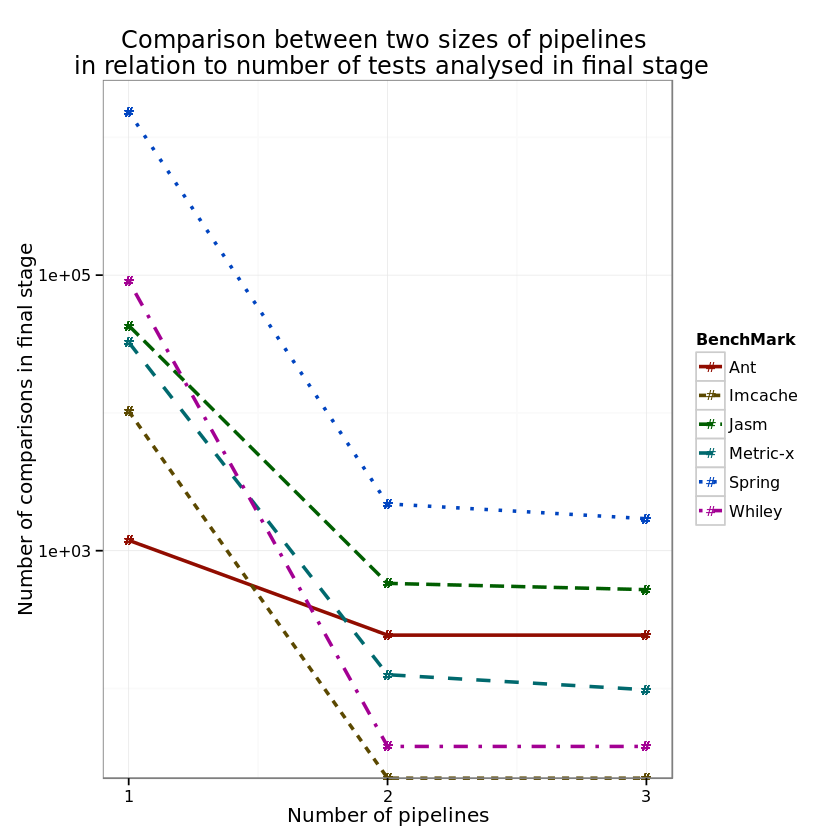
\includegraphics[height=10cm, width = 14.5cm]{Pipeline.png}
\end{center}
\caption{A figure showing the effect that using pipelines has on the number of comparisons that the final stage (Most computationally heavy) has to do.}
\label{fig:pipelinegraph}
\end{figure}


\section{K Length Comparison}

Figure \ref{fig:kdepthgraph} shows the change that the KDepth had on the number of redundant test cases identified. \todo{Should I do sig test? It would mean I have to write more code to do it}

\begin{figure}[H]
\begin{center}
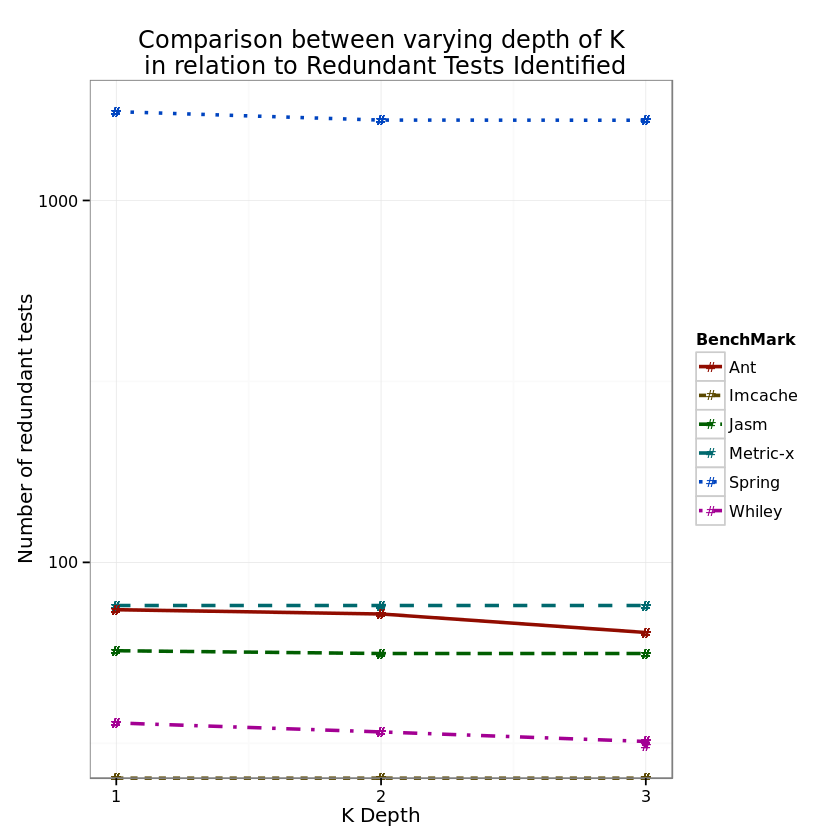
\includegraphics[height=10cm, width = 14.5cm]{KDepth.png}
\end{center}
\caption{A figure showing the effect that a change in the depth of the calling context has on the number of redundant tests are identified.}
\label{fig:kdepthgraph}
\end{figure}

\section{Parameter Comparison}

The significant table for comparing the use of parameters is shown in Table \ref{parametersig}. It shows that there was a negative relation for every benchmark in regard to time taken, this shows that parameters caused an increase in the time taken to analyse the data. Every benchmark had a significantly positive effect on the number of redundant test cases identified, showing that parameters decrease the number of redundant test cases. This is not the case in Imcache due to it having 0 redundant test cases identified in both, therefore no difference between the two.


\begin{table}[h]
\centering

\label{parametersig}
\begin{tabular}{|l|l|l|}
\hline
{\bf }          & {\bf Total Time} & {\bf Redundant Tests Identified} \\ \hline
{\bf Whiley}    & +                & -                           \\ \hline
{\bf Jasm}      & +               & -                          \\ \hline
{\bf Ant}       & +                & -                           \\ \hline
{\bf Spring}    & +                & -                           \\ \hline
{\bf Imcache}   & +                & =                           \\ \hline
{\bf Metrics-x} & +                & -                           \\ \hline
\end{tabular}
\caption{A table showing the significant relationship between the use of parameters and no parameters for each benchmark}
\end{table}

\begin{figure}[h]
\begin{center}
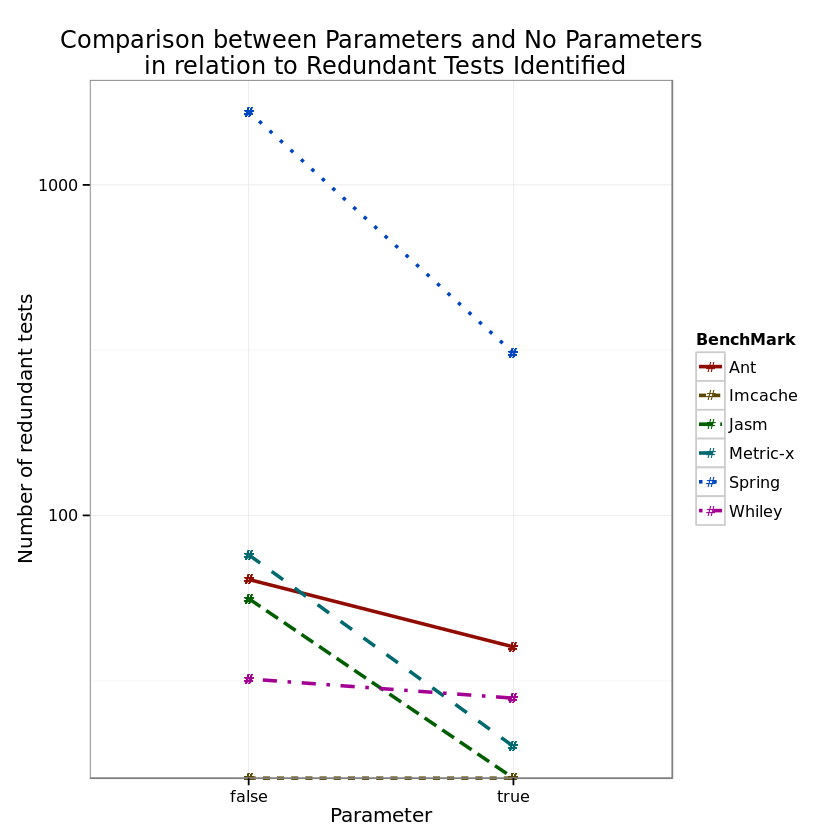
\includegraphics[height=10cm, width = 14.5cm]{Parameters.png}
\end{center}
\caption{A figure showing the effect that using parameters has on the number of redundant tests are identified.}
\label{fig:paramgraph}
\end{figure}

\section{Weighting Comparison}

The significant table for comparing the use of weighting is shown in Table \ref{weightingsig}. There are a mix for the benchmarks in regard to the total time taken to analyse the data. Whiley, Ant and Imcache had a significantly negative relation and weighting increased the time taken to analyse. Jasm, Spring and Metric-x had a significantly positive relation and weighting decreased the time taken to analyse. Whiley, Ant, Jasm and Metrics-x had a significantly positive relation in regard to the number of redundant tests identified, showing a decrease in the number identified when weighting was applied. Spring was the only benchmark where weighting had a significantly negative impact, increasing the tests identified.

\begin{table}[h]
\centering

\label{weightingsig}
\begin{tabular}{|l|l|l|}
\hline
{\bf }          & {\bf Total Time} & {\bf Redundant Tests Identified} \\ \hline
{\bf Whiley}    & +                & -                           \\ \hline
{\bf Jasm}      & -                & -                           \\ \hline
{\bf Ant}       & +                & -                           \\ \hline
{\bf Spring}    & -                & +                           \\ \hline
{\bf Imcache}   & +                & =                           \\ \hline
{\bf Metrics-x} & -                & -                           \\ \hline
\end{tabular}
\caption{A table showing the significant relationship between the use of weighting and no weighting for each benchmark}
\end{table}


\begin{figure}[h]
\begin{center}
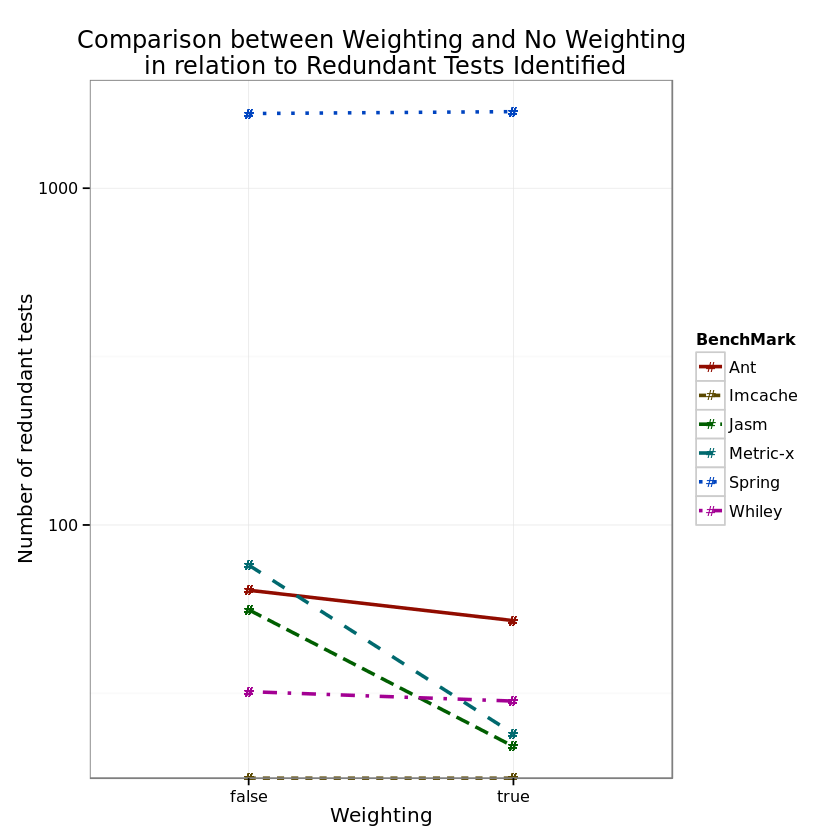
\includegraphics[height=10cm, width = 14.5cm]{Weighting.png}
\end{center}
\caption{A figure showing the effect that using weighting has on the number of redundant tests are identified.}
\label{fig:weightgraph}
\end{figure}

\section{Weighting and Parameter Comparison}

The significant table for comparing the use of weighting with parameters is shown in Table \ref{weightingparamsig}. It shows that for every Benchmark apart from Imcache, there was a negative relation for the time taken, showing that the time increased when using weighting and parameters for the majority of benchmarks. In contrast to this, every benchmark had a positive relation to the number of redundant tests identified.

\begin{table}[h]
\centering
\label{weightingparamsig}
\begin{tabular}{|l|l|l|}
\hline
{\bf }          & {\bf Total Time} & {\bf Redundant Tests Identified} \\ \hline
{\bf Whiley}    & +                & -                           \\ \hline
{\bf Jasm}      & +                & -                           \\ \hline
{\bf Ant}       & +                & -                           \\ \hline
{\bf Spring}    & +                & -                           \\ \hline
{\bf Imcache}   & -                & =                           \\ \hline
{\bf Metrics-x} & +                & -                           \\ \hline
\end{tabular}
\caption{A table showing the significant relationship between the use of weighting with parameters and neither for each benchmark}
\end{table}

\begin{figure}[h]
\begin{center}
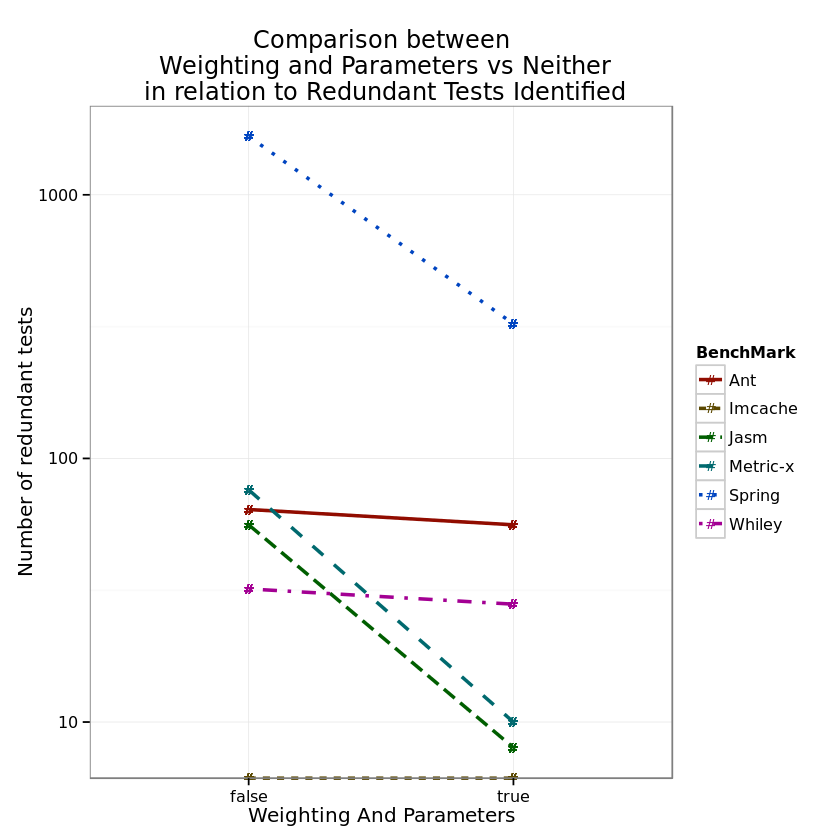
\includegraphics[height=10cm, width = 14.5cm]{WeightNParam.png}
\end{center}
\caption{A figure showing the effect that using weighting and parameters has on the number of redundant tests are identified.}
\label{fig:weightingparamgraph}
\end{figure}

\section{Redundant Test Case Coding}

Table \ref{whileycoding} compares the four major variations of techniques used to show the different types of redundancy that were picked up for the Whiley benchmark. 

\begin{table}[h]
\centering
\label{whileycoding}
\begin{tabular}{|l|l|l|l|l|}
\hline
                          & \multicolumn{4}{c|}{{\bf Whiley}}                                                             \\ \hline
{\bf Types of redundancy} & \multicolumn{1}{c|}{{\bf Pipeline 2}} & {\bf Weighting} & {\bf Parameters} & {\bf Parameters \& Params} \\ \hline
Different Equation Value  & 6                                     & 6               & 6                & 6                \\ \hline
Different Equation Sign   & 8                                     & 8               & 8                & 8                \\ \hline
Different Array Values    & 2                                     & 2               & 0                & 0                \\ \hline
Same                      & 10                                    & 10              & 10               & 10               \\ \hline
Limited Redundancy        & 2                                     & 0               & 0                & 0                \\ \hline
Rearranged Equation       & 2                                     & 2               & 2                & 2                \\ \hline
Extra if statement        & 2                                     & 2               & 2                & 2                \\ \hline
                          &                                       &                 &                  &                  \\ \hline
{\bf Total}               & 32                                    & 30              & 28               & 28               \\ \hline
\end{tabular}
\caption{A table displaying a list of coding's for the Whiley Benchmark for four of the different techniques used.}
\end{table}